% Multumiri lui Gabriel Majeri, acest sablon a fost creat pe baza
% codului sursa a lucrarii sale de licenta. 
% Codul sursa: https://github.com/GabrielMajeri/bachelors-thesis
% Website: https://www.gabrielmajeri.ro/
%
% Aceast sablon este licentiat sub Creative Commons Attribution 4.0 International License.

\documentclass[12pt, a4paper]{report}

% Modificarea geometriei paginii
\usepackage{geometry}
\geometry{
    margin=2cm
}

% Suport pentru diacritice și alte simboluri
%\usepackage{fontspec}

% Suport pentru mai multe limbi
\usepackage{polyglossia}

% Setează limba textului la engleză
\setdefaultlanguage{english}

% Suport pentru diferite stiluri de ghilimele
\usepackage{csquotes}

% Utilizează biblatex pentru referințe bibliografice
\usepackage[
    maxbibnames=50,
    sorting=nty,
    backend=biber,
    style=numeric
]{biblatex}

\addbibresource{bibliography.bib}

% Setează spațiere inter-linie la 1
\usepackage{setspace}
\singlespacing

% Include funcțiile de grafică
\usepackage{graphicx}
% Încarcă imaginile din directorul `images`
\graphicspath{{./images/}}

% Listări de cod
\usepackage{listings}

% definirea culorilor
\usepackage{xcolor}

\definecolor{codeblue}{rgb}{0.11, 0.56, 1}
\definecolor{codegold}{rgb}{0.8, 0.64, 0}
\definecolor{codegray}{rgb}{0.3, 0.3, 0.3}
\definecolor{codepurple}{rgb}{0.7, 0.5, 0.7}

\lstdefinestyle{mystyle}{
    commentstyle=\color{codepurple},
    keywordstyle=\color{codeblue},
    numberstyle=\tiny\color{codegray},
    stringstyle=\color{codegold},
    basicstyle=\ttfamily\footnotesize,
    breakatwhitespace=false,         
    breaklines=true,                 
    captionpos=b,                    
    keepspaces=true,                 
    numbers=left,                    
    numbersep=5pt,                  
    showspaces=false,                
    showstringspaces=false,
    showtabs=false,                  
    tabsize=2
}

\lstset{style=mystyle}

% Linkuri interactive în PDF
\usepackage[
    colorlinks,
    linkcolor={black},
    menucolor={black},
    citecolor={black},
    urlcolor={blue}
]{hyperref}

% Simboluri matematice codificate Unicode
\usepackage[warnings-off={mathtools-colon,mathtools-overbracket}]{unicode-math}

% Comenzi matematice
\usepackage{amsmath}
\usepackage{mathtools}

% Formule matematice
\newcommand{\bigO}[1]{\symcal{O}\left(#1\right)}
\DeclarePairedDelimiter\abs{\lvert}{\rvert}

% Suport pentru rezumat în două limbi
% Bazat pe https://tex.stackexchange.com/a/70818
\newenvironment{abstractpage}
  {\cleardoublepage\vspace*{\fill}\thispagestyle{empty}}
  {\vfill\cleardoublepage}
\renewenvironment{abstract}[1]
  {\bigskip\selectlanguage{#1}%
   \begin{center}\bfseries\abstractname\end{center}}
  {\par\bigskip}

% Suport pentru anexe
\usepackage{appendix}

% Stiluri diferite de headere și footere
\usepackage{fancyhdr}

\fancypagestyle{main}{
  \fancyhf{}
  \renewcommand\headrulewidth{0pt}
  \fancyhead[C]{}
  \fancyfoot[C]{\thepage}
}

% Metadate
\title{Paging with Dynamic Memory Capacity \\ \LARGE -- Summary --}
\author{Radu Ștefan-Octavian}

% Generează variabilele cu @
\makeatletter

% nu folosi indentare ci spatiere intre paragrafe
\usepackage[parfill]{parskip}

\begin{document}

% Main matter
\cleardoublepage
\pagestyle{main}
\let\ps@plain\ps@main

\begin{titlepage}

% Redu marginile
\newgeometry{left=1cm,right=1cm,bottom=1cm}

\begin{figure}[!htb]
    \centering
    \begin{minipage}{0.2\textwidth}
        
\includegraphics[width=\linewidth]{logo-ub.png}
    \end{minipage}
    \begin{minipage}{0.5\textwidth}
        \large
        \vspace{0.2cm}
        \begin{center}
            \textbf{UNIVERSITATEA DIN BUCUREȘTI}
        \end{center}
        \vspace{0.3cm}
        \begin{center}
            \textbf{
                FACULTATEA DE \\
                MATEMATICĂ ȘI INFORMATICĂ
            }
        \end{center}
    \end{minipage}
    \begin{minipage}{0.2\textwidth}
        
\includegraphics[width=\linewidth]{logo-fmi.png}
    \end{minipage}
\end{figure}

\vspace{5cm}

\begin{center}
\huge \textbf{\@title}\\
\end{center}

\vspace{3.5cm}

\begin{center}
\large \textbf{Student \\ \@author}
\end{center}

\begin{center}
\large \textbf{Scientific coordinator \\ Prof. Dr. Alexandru Popa}
\end{center}

\vspace{2.5cm}

\begin{center}
\normalsize \textbf{Bucharest, December 2022}
\end{center}
\end{titlepage}

\chapter{Introduction}

\section{Motivation}

\section{Idea}

\section{Contribution}

\section{Outline}

\chapter{Background}


%TODO other things to add:
%* blocks
%* opcodes
%* CFG

In this chapter we will cover concepts relevant for the rest of the paper. %TODO continue

\section{Malware}

The word \emph{malware} is a blend word for malicious software. As such, it is an umbrella term which encompasses any type of software which is intentionally designed to disturb the intended use, or operation of a computer system, without the explicit permission of its user(s) or owners. The goal of a piece of malware can include, but is not limited to: leakage or collection of private information, restriction of access to data with the goal of monetary gains, network overload, device hijacking, espionage, serving of targeted adds \cite{wiki_malware}.

\subsection{Classification}

Malware are typically grouped by their behaviour and/or purpose and could fall under one or more of the labels in the following non-exhaustive list: backdoor, bot(net), dropper, fileless, ransomware, rootkit, spyware, trojan, virus, worm, etc. We will shortly cover the most relevant ones as follows \cite{wiki_malware}, \cite{zeusvm}.

\subsubsection{Backdoor}

A Backdoor is an umbrella term depicting programs that enable bad actors to obtain persistent, unauthorised access on a victim's computer, typically without them being aware of the situation. Backdoor are interesting, because they can either be delivered through a Trojan, a worm, or another similarly purposed malware, but they can also be the result of vulnerabilities existing in legitimate software, that already exist on the victim's computer. What is more, there also a combined scenario, where a backdoor is intentionally inserted into legitimate software. This can be done, for instance, by a bad actor hiding their intension. This was the case, for instance, with the 2024 discovery of the XZ Utils backdoor \cite{xz_backdoor}.

\subsubsection{Trojan}

A Trojan, or a Trojan Horse, is a type of malware that concals itself inside another program that appears benign. It typically misinforms the target about its behaviour in order to persuade a victim to install it on their computer. Trojans are usually delivered by some form of social engineering. The payload of a Trojan can be anything. It often is another type of malware, case in which, the Trojan is considered a Dropper. It can also be the case that the Trojan deploys a backdoor which can enable unauthorised control of the infected system to a third party actor.

\subsubsection{Worm / Virus}

Worms and viruses are simmilar in the sense that these are both standalone malware that have the capacity to spread through a network, and to infect other victims. A virus (inspired from the biologial term) will inject itself simmingly harmless programs, which upon execution will further spread the infection. Worms differ from viruses in the sense that a virus requires the victim to execute the infected software in order for it to spread, whereas a worm does not. Worms can spread without user intervention and without modifying other files on the system \cite{wiki_malware}. An example of such a piece of malware is the infamous Stuxnet virus \cite{stuxnet}.

\subsubsection{Ransomware}

Ransomware is a type of malware that, once it infected a computer, restricts access to information on that particulat machine, and then requires a ransom from the victim, in exchange from the locked up information. Most comonly, a form of encryption is applied to the restricted data, which in properly executed attacks cannot be recovered without the encryption key. Typically, ransomware is delivered via a Trojan, but this is not always the case. The infamous \emph{WannaCry} ransomware was a \emph{worm} which spread through the network without user intervention \cite{wiki_wannacry}, \cite{wiki_ransomware}. As it can be seen in Figure \ref{fig:wannacry}, the attackers will ask for hard to trace digital currencies, such as Bitcoin in this case.

\begin{figure}[h]
    \centering
    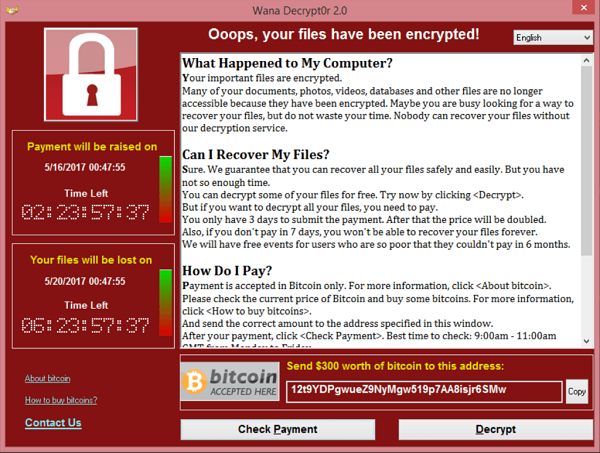
\includegraphics[width=0.8\textwidth]{./images/wanacry.png}
    \caption{TODO}
    \label{fig:wannacry}
\end{figure}

\subsubsection{Bot and Botnets}

A bot is a computer infected by a specific type of malware which enables its victim to be remotely controlled. Such malware is spread with the goal of infecting as many targets as possible. The infected machines are added to a common pool, called a \emph{botnet}, which can be orchestrated from a \gls{CC} center to perform other malicious activities on a bigger scale. The Andromeda botnet is an example of such malware \cite{andromeda} \cite{kaspersky_malware_types}.

\subsection{Relevance}

Malware attacks, which we will further refer to with the broader term of cybercrime, can target governments, corporations, public figures, or individuals. Multiple sources, including a report from the World Economic Forum \cite{wef_cybercrime}, suggest that cybercrime continues to rise both in numbers as well as in damage. The estimated costs of cybercrime in 2023, at a global scale, are of \$11.5 trillion, and these numbers are expected to more than double in the next 5 years. Because of this, malware, and particularly the subject of malware analysis, are evermore relevant.

\section{Reverse Engineering} % TODO obv change this
% TODO get a glossary going
% TODO glossary list:
% * reverse engineering

% TODO: this passage is nice : > Also, a discipline that may be used to any area of forward engineering; it is analogous to scientific research except that the study is performed on a man-made product rather than a natural event.

As stated on \emph{Wikipedia}: \emph{``Reverse engineering is a process or method through which one attempts to understand through deductive reasoning how a previously made device, process, system, or piece of software accomplishes a task with very little (if any) insight into exactly how it does so''} \cite{re_wiki}.
% TODO maybe give more context into historical examples of reverse engineering and how they benefited society: hierogliphs, russian plane, telescope, IBM pc, etc.

% TODO define malware

In this work we will focus on reverse engineering pieces of software in the context of performing security research or malware analysis. Typically, in such contexts, the goal is to understand the behaviour of a piece of software, without having access to its source code. Depending on the type of analysis, a reverse engineer might have different approaches. 

They might focus on gaining a comprehensive understanding of specific parts of the software in order to identify weaknesses, or more commonly named \emph{vulnerabilities}. The analysis could be restricted to specific parts because for multiple reasons which include, but are not limited to: the full program being to big to justify performing a full analysis, or the existence of prior knowledge which gives higher priority to the analysis of certain code regions. With the knowledge obtained from RE, the engineer can identify and prove the existence of attack vectors on a system that is running this software. They might then write a report which covers the risks to which entities running the software are exposed, describing in detail the finding and, eventually exemplifying how an attacker might abuse the discovered vulnerabilities. In this case, the end goal is to initiate the process of patching the vulnerable piece of software. % TODO might want to cite here

In other instances, the engineers might perform a full and comprehensive analysis of piece of software. This is typically done when dealing with malware. The malware analyst will first try to determine if the piece of software is in fact malicious or not. If the code is malicious, it is important to determine its behaviour, how it interacts with the system, or with outside entities (possibly by creating network traffic). Further, analysts might study and document novel techniques employed by attackers. They might also integrate the newly find malware into a detection system to prevent future uses of the respective malware \cite{malware_crowdstrike}.

Regardless of the goal, RE falls into one of two broad categories which determine the typical approach and the tooling used: \textbf{static analysis} and \textbf{dynamic analysis}.

\section{Static Analysis}

Static analysis represents the multitude of techniques employed to analyse a program without executing it. These techniques range in difficulty and complexity starting from reading source code, to reading assembly, attempting to decompile the binary and ultimately to using very advanced tools and theoretical knowledge such as \gls{SE} engines, SMT solvers or formal methods. %TODO I am not sure anylonger if SE should be included here or not

In its most basic form, static analysis is equivalent with reading the source code in order to understand what the program does. However, in the context of this paper, we are dealing with binary files, compiled to machine code. The source code is not available to us, so we must resort to other analysis techniques. One option is to convert the machine code into the human readable form, called assembly. The process is known as machine code disassembly. Assembly code is typically very hard to understand for humans, but from it the logic of the program can be successfully recovered, given enough time and effort. One advantage of static analysis through reading assembly is that the entry barrier is not high in terms of the tooling required. A very basic tool such as \cc{objdump} \cite{TODO} can be enough for simple programs, but most likely a more feature rich tool such as \cc{radare2}/\cc{cutter} \cite{TODO} might be more suitable, as these are able to display basic blocks and how all such basic block(BB TODO) relate to each other and form the Control Flow Graph(CFG TODO).

Reverse engineers typically default to more advanced static analysis tools, such as IDA or Ghidra. These tools feature a suite of functionalities, out of which, probably the most prominent is the \emph{decompiler}. Compilation is the process of converting source code into machine code. Decompilation is the opposite: the process of converting machine code, back into source code. Compared to the disassembly process, which is deterministic and corresponds exactly to the assembly process, the decompilation process will almost never yield back the original source code. This is the case because a lot of information useful to programmers, but useless for the CPU(TODO) is lost during the compilation process. This information includes, but is not limited to: variable and function names, type information, custom defined data types such as structures, or specific language features. This is why decompilers will always output an approximation of the original code. 

Let us consider a concrete example and consider Listings \ref{code:decompilation-original}, \ref{code:decompilation-1}, \ref{code:decompilation-2}. Listing \ref{code:decompilation-original} contains the implementation of the function \cc{add}, which takes the end of linked list and a value, and creates a new node in the list with that value, also taking the necessary steps to update the list accordingly. The code is part of a slightly larger \cc{C} program, which we compiled and imported into Ghidra. Looking at Listing \ref{code:decompilation-1} we can see the decompilation of the exact code in the previously mentioned listing. It is immediately obvious that: the type information related to \cc{node} structure is completely lost and that the original function was inlined by the compiler. As a result, the decompilation is an obfuscated version of the original code. This is a well known fact and advanced tools such as Ghidra offer various features, which the reverse engineer can utilise in order to remove part of the obfuscation. Listing \ref{code:decompilation-2} contains the same segment of decompiled code after a minimal amount of manual intervention, which includes: variable renaming, custom type creation and type updates. Clearly, it is a lot more human readable and bears a closer resemblance to the original code in Listing \ref{code:decompilation-original}. 

Decompilers and disassemblers are very powerful tools, which aid significantly in the process of static analysis. However, these tools have their shortcomings as highlighted above. Moreover, there are certain program behaviours which cannot, or are significantly harder to understand only by \emph{looking} at the code.

% Found a paper which I can use to add more about this :D
% see static analysis techniques 2015

% TODO mention techniques which hinder static analysis

% TODO set vspace / margin before listings
\begin{lstlisting}[language=c, label={code:decompilation-original}, caption={TODO}]
void add(lnode** node, int v) {
    // allocate memory for a new node in the liked list
    lnode* new_node = (lnode*) malloc(sizeof(lnode));
    new_node->val = v; // set the value
    if (*node != NULL) {
        (*node)->nxt = new_node; // link to the new node from the end of the list
        *node = new_node; // move the list end to the new node
    } else {
        *node = new_node; // TODO fix comments set it as the end of the list, it it is the first one
    }
}
\end{lstlisting}

% TODO i'd like to try to get two columns in here
\begin{lstlisting}[language=c, label={code:decompilation-1}, caption={TODO}]
piVar1 = (int *)malloc(0x10);
*piVar1 = iVar3;
if (piVar5 != (int *)0x0) {
    *(int **)(piVar5 + 2) = piVar1;
}
piVar5 = piVar1;
if (piVar4 == (int *)0x0) {
    piVar4 = piVar1;
}
\end{lstlisting}

\begin{lstlisting}[language=c, label={code:decompilation-2}, caption={TODO}]
new_node = (node *)malloc(0x10);
new_node->val = v;
if (last_node != (node *)0x0) {
    last_node->nxt = new_node;
}
last_node = new_node;
if (root == (node *)0x0) {
    root = new_node;
}
\end{lstlisting}

\section{Dynamic Analysis}

As described by T. Ball in his 1999 paper \cite{concept_of_da_1999}, \emph{``dynamic analysis is the analysis of a running program''}. This type of analysis is desirable in different situations where static analysis could not extract sufficient information, or when acquiring extra information depends the program to be running %TODO i could give more examples here, relating to why static analysis cannot work in certain situations. also should mention for the static analysis part exactly this. probably will need to talk before RE about obfuscation techniques. OR NOO!! I can talk right after, in order to present some means to prevent static analysis
Dynamic analysis is an umbrella term which covers many powerful techniques used for program analysis. A taxonomy of these techniques has been presented in a comprehensive survey by Ori et al. in 2019 \cite{da_survey_2019}. We will shortly cover some of them.

\subsection{Debugging}

% TODO define somewhere that we'll be referring to a reverse engineer / malware analysit as "the analyst" throughout this work

Debugging is a very well known technique, especially popular among developers who use it mainly to identify bugs or errors in their code. It is however a very effective and reliable form of analysing unknown programs (eg. malware). Also called \emph{single stepping}, it involved using a tool, intuitively called a \emph{debugger}, in order to run the program one instruction at a time. After each instruction, the analyst can inspect the state of the registers, the memory and what instructions follow. This process can also help in determining any relevant changes in the operating system itself, caused or related to the debugged program.

Debuggers use the CPU's trap flag in order to trigger an interrupt after each instruction, or only certain desired instructions. The interrupt causes a context switch from the execution of the debugged program to the debugger. To continue execution, the trap flag is set again and the context switches back to the program. The high number of context switches means that debugging is a very resource intensive analysis technique. It is also very easy to detect by the running malware, which can check the state of the trap flag and hide its behaviour in case it is debugged \cite{da_survey_2019}.

\subsection{Function Call Analysis}

% TODO explain what a syscall is?

Any type of meaningful action that a malware can take, will ultimately rely on system calls. It can be the case that these system calls are performed through function calls from an external library, such as the standard \cc{libc} library, or from an internally defined function. Analysing function calls, the state of the program before, during and after the function call, as well as the parameters used can provide valuable information about the behaviour of the analysed program. Techniques for approaching this goal vary. For instance, we could use command line (cli TODO) programs such as \cc{strace}, or \cc{ltrace}, which track system calls and library calls respectively. We could also use more advanced techniques, such as function hooking. An analyst can extract more information from a function call by \emph{hooking} (i.e. linking) a piece of code to the targeted function. What will happen is that upon the function call, the \emph{hooked} code will run as well, which can just print debugging messaged to inform the analyst that the function has just been called, or access the state of the program at that time and save it for further inspection. \cite{da_survey_2019}

Function calls can also be used as a powerful side-channel. More specifically, one can monitor the amount of \cc{calls} which have been made since reference point in order to determine if progress has been made or not in the execution. Let's consider Listing \ref{code:ltrace}. We're running the \cc{crackme} program through \cc{ltrace} to monitor function calls, with a randomly chosen input string. We notice a length check with \cc{strlen} at Line \ref{code:ltrace-1}, after which the program crashes. By selecting the correct input length of $70$ bytes, we can pass the length check at Line \ref{code:ltrace-2}. This \cc{crackme} is a particularly good example for using this technique, because it is heavily obfuscated. We cannot effectively use static analysis on this binary, so employing dynamic analysis techniques enables us to make progress and recover the secret \cite{crusu_relabs}.

% TODO explain what a crackme is 

\begin{lstlisting}[caption={TODO}, label={code:ltrace}]
>_ python -c "print('a' * 42)" | ltrace ./crackme
memset(0x8625ae8, '\0', 10000)                         = 0x8625ae8
fgets("aaaaaaaaaaaaaaaaaaaaaaaaaaaaaaaa"..., 10000, 0xf22e9700) = 0x8625ae8
strlen("aaaaaaaaaaaaaaaaaaaaaaaaaaaaaaaa"...)          = 43 @$\label{code:ltrace-1}$@
puts("WROOONG!"WROOONG!)                               = 9
exit(1 <no return ...>)
+++ exited (status 1) +++

>_ python -c "print('a' * 70)" | ltrace ./crackme
memset(0x8625ae8, '\0', 10000)                         = 0x8625ae8
fgets("aaaaaaaaaaaaaaaaaaaaaaaaaaaaaaaa"..., 10000, 0xedcf4700) = 0x8625ae8
strlen("aaaaaaaaaaaaaaaaaaaaaaaaaaaaaaaa"...)          = 71
strstr("aaaaaaaaaaaaaaaaaaaaaaaaaaaaaaaa"..., "zihldazjcn") = nil @$\label{code:ltrace-2}$@
puts("WROOONG!"WROOONG!)
exit(1 <no return ...>)
\end{lstlisting}

\subsection{Fuzzing}

\subsection{Dynamic Taint analysis}

Dynamic Taint analysis is a technique used to track data flow from sources to sinks. In order to achieve this goal, data considered important is given a label (\emph{a taint}), based on a \emph{taint introduction policy}. Typically, we would taint untrusted user input or data arriving over the network. This \emph{tainted} data is propagated through the system based on execution and how the code interacts with the data at the opcode level. When an operation is performed on tainted data, memory locations used during the respective operation are also tainted, based on a \emph{taint propagation policy}. Some memory areas, or code sections are also marked as \emph{sinks}. When tainted data arrived at a sink, the path it took through the code can be traced back. In the context of malware analysis, the flow of tainted data is valuable, as it gives valuable insights about the ways the malware interacts with the user and the operating system. Taint analysis is also valuable for exploit detection, and was initially used specifically for this goal. By tainting untrusted user input one can detect unusual data flows and detect attempts at exploiting a system. In such cases, a \emph{taint checking policy} might be used to determine further behaviour (e.g. halting execution) \cite{da_survey_2019} \cite{all_about_taint_2010}.

\section{Other Approaches}

\subsection{Symbolic Execution}

\gls{SE} is a powerful program analysis technique, and one of the core techniques which the idea of this paper is based on. As such, we will cover \gls{SE} in more detail compared to the other dynamic analysis approaches.

% TODO bat campii efectiv, trebuie sa reformulez
\gls{SE} is typically discussed in relation with \emph{\gls{CE}}. \gls{CE} is the formal term for what we refer to as normal program execution. That is, executing a program with a concrete input until the end of a single execution path. When every possible external value (user input, response from a system call, return value of a function) has a concrete value, we're dealing with \gls{CE}.
Let us consider Listing \ref{lst:fizzbuzz}. The value of the argument \cc{c} is given by the caller of the function \cc{fizzbuzz}. If we consider a concrete value of $7$ for \cc{c}, we expect the program to print the same value $7$ at the standard output, after executing Line \ref{code:fizzbuzz-1}. We can test this hypothesis by running the program, passing the respective value to the function and inspecting the printed value. This is concrete execution.

\lstinputlisting[language=c, label={lst:fizzbuzz}, caption={TODO}]{./code/fizz-buzz.tex}

In contrast with \gls{CE}, with \gls{SE} we can explore all possible paths of execution. Moreover, for each path we will have a logical condition which precisely describe the values of the inputs which will lead the execution on that specific path.

in order to determine what classes of inputs lead to which execution paths.

The key aspect of \gls{SE} is the use of symbolic values, as opposed to concrete values. Initially, the symbolic values are unconstrained, meaning that they can represent any possible input value associated to that type. The program is executed in a controlled environment by a \gls{SE} engine. The engine keeps track of a logic formula which describes the constraints that the input must satisfy, in order to follow each specific execution path that is being tracked. It also keeps trace of the symbolic memory store, which keeps track of symbolic values and memory areas, and the expressions or concrete values which these hold. As the program executes, each conditional branch splits the symbolic state into two and adds new constraints to each branch, based on the respective conditional.

\subsection{Concolic Execution} % \subsection{Mixed Approaches ???}

% TODO this paragraph does not fit here AT ALL!
% TODO find a way to repurpose it
% Typically, when running unknown software the researcher or analyst is exposing his system to the risk of being compromised. This is especially prevalent when we are dealing with potential malware. For these situations specific techniques have been devised in order to protect the host system from being infected, while still having an environment where the unknown software can be executed and its interactions with the system monitored and then analysed. Such environments are called sandboxes, and isolate the suspicious software from the main OS(TODO), in such a way that the host of the system, as well as the network are safe from infection, or compromise.

%\section{Malware Obfuscation}
\section{Obfuscation Techniques}

% TODO cite more, provide source for evading protections

Obfuscation is an umbrella term for a set of techniques, very widely employed in the field of software engineering, for protecting source code. This is done by making the code harder to understand, without changing its behaviour (semantics). Obfuscation is used, especially when the code contains \gls{PI}, which must be protected against \gls{RE}. Not surprisingly, obfuscation is very common in malware. In this case, obfuscation is used to evade automatic malware detection systems, such as anti-viruses. Moreover, many obfuscation techniques are specifically aimed at the researchers who are expected to attempt doing \gls{RE} on it, aiming to slow down the analysis, which in turn enables the bad actors to inflict more damage on their targets. \cite{zeusvm} 

\subsection{Classification}

There are a number of malware obfuscation techniques which have been observed in the wild time and time again. We will cover some of the most relevant as follows

\subsubsection{Classical Techniques}

%\subsubsection{Encryption}
%\subsubsection{Constant Unfolding}
%\subsubsection{Dead Code Insertion}
%\subsubsection{Data encoding schemes}
%\subsubsection{Pattern-based obfuscation}
%\subsubsection{Control Indirection}
%\subsubsection{Junk Code insertion}

% FIXME I hate you!!!!!

A very common way to try and evade signature-based detection is to encrypt the malicious payload. This obfuscation technique implies a couple of things. First of all there needs to exist an encryptor, which encrypts each iteration of the malware, ideally with a different key. As such the result differs between iterations. Second of all, there needs to exits a decryptor, packaged together with the malware. This is essential, because the decryptor must be triggered upon execution of the malicious code, in order for the operating system to be able to execute it. The second point constitutes a big weakness of this technique, because the antivirus could employ a strategy where it targets the signature of the decryptor.

% TODO very much to do here !!
\subsubsection{Classical Techniques}

\subsubsection{Opaque Predicates}

\subsubsection{Control-Flow Flattening}

\subsubsection{Mixed Boolean-Arithmetic}
% TODO there is a paper somewhere about this one

\subsubsection{Virtual Machines}

\cite{malware_obf}
% TODO it is important to note that techniques are not singluar and can, and often are, combined


% TODO figure out if this fits better in the next chapter (I think yes)

\Glspl{VM} 

\chapter{Our approach}

%i THINK i SHOULD GET STARTED ON WRITING ABOUT OUR APPROACH, AND DISCUSS EVERYTHING THAT i HAVE DONE AND USED THROUGHOUT THE EXPERIMENTS. iT IS GENUINELY A WASTE OF TIME TO WORK ON THE FKING BACKGROUND SECTION AND ON THE sota AND READ PAPERS AFTER PAPERS ONLY TO GET MORE DEPRESSED BECAUSE MY APPROACH SUCKS COMPARED TO WHAT i'M READING IN THE ACADEMICS

\section{Overview}

In this thesis we target the problem of reverse engineering binaries obfuscated with the embedded \glspl{VM} technique. We propose a couple of improvements to classical techniques for this specific problem, using modern tools. Namely, the core idea is to enable symbolic execution of the VM bytecode, through the angr framework \cite{TODO}. To do this, we propose creating an angr plugin, for a specific VM architecture, which would enable (almost) all of angr's analysis features to be applied on that specific architecture. We build on top of this and propose \cc{arch-genesis}, a tool which simplifies the process of creating a new architecture plugin, by abstracting away most of the boilerplate code, and allowing the user to focus only on the core logic of the \gls{VM}. We, then show how this plugin can be used as a decompiler, and for control-flow graph generation. Throughout, we employ various other well known techniques, such as static analysis, using well known tools such as Ghidra. We also discuss lesser known techniques for recovering the semantics of the \gls{VM} handlers.

% Check the paragraph below if it makes sense
To exemplify the way in which our method can be applied, we solve 2 \gls{CTF} challenges of different difficulties. These challenges propose \gls{ELF} binaries, obfuscated using embedded \glspl{VM} to be reverse engineered. Although the chosen samples do not accurately resemble real world malware, they serve as a solid entry point into malware reverse engineering and \gls{VM}-based obfuscation. In the following sections we present the process of reverse engineering the mentioned binary files and the corresponding \glspl{VM}. We end this chapter with a discussion on the advantages and the shortcoming of our approach, based on our experience with the two samples, as well as other real-world samples. We end with future directions.

The two analysed binary files were part of the 2023 UIU CTF (the \cc{vmwhere} challenge) \cite{TODO} and the 2023 Imaginary CTF (the \cc{vmcastle} challenge), in the \gls{RE} category. The challenges were solved during the competition by the top 8\% and top 2\% of the teams, respectively.

\subsection{Assumptions}

% TODO not sure if this is useful in any way to mention
It is relevant to note some assumptions that we made in our analysis use-case:
* we're dealing with understanding the behaviour of the bytecode, and are not so
interested in the actual reverse engineering process of the interpretor. * we


assume that the logic of the interpretor was, or can be recovered through


reasonable means, despite various obfuscation techniques that might have been
applied 
%* idk??


\section{Understanding the VM}

In order to integrate a new architecture into angr, we need to understand the structure of the \gls{VM}, and what each of the \gls{VM} handlers does. For this, we rely on both on static analysis using Ghidra \cite{TODO}, as well as a lesser known technique which uses symbolic execution for simplifying the logic of the handlers, using the \emph{Miasm} framework \cite{TODO tim blog}.

\subsection{Static Analysis}

We begin by opening the binary file in Ghidra \cite{TODO}, an open source \gls{RE} framework, developed by the \gls{NSA}. Despite its dated looks and clunky \gls{UI}, Ghidra features not only a power disassembler, but numerous other features, such as \gls{CFG} representation, and a very powerful decompiler. We use it to quickly identify the source of the bytecode, which is the \gls{stdin}: the file path of a file containing the \gls{VM} bytecode is passed to \gls{stdin} in both cases, after which it is parsed and passed onwards to the bytecode interpretor. We continue the analysis with this interpretor, which is the interesting part of the program.

\begin{figure}[h]
    \centering
    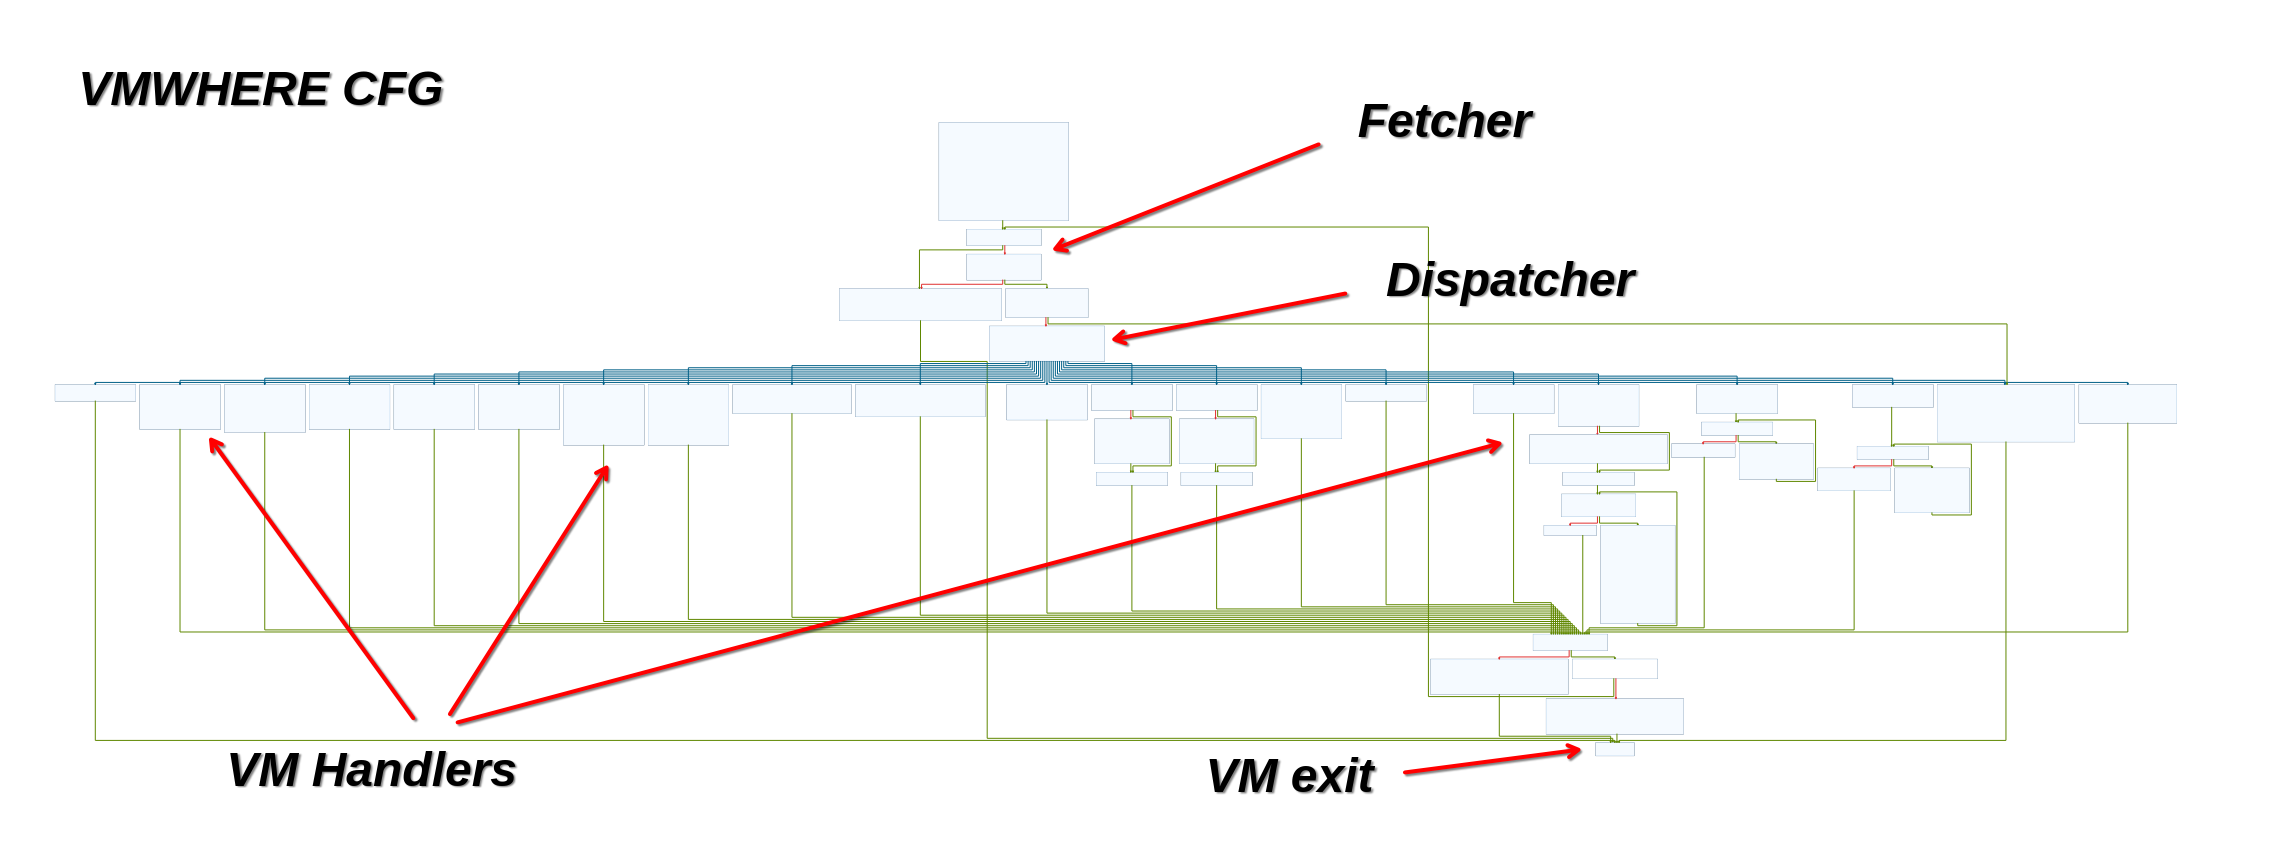
\includegraphics[width=\textwidth]{./images/cfg_vmwhere}
    \caption{TODO, but also mention that you used Cutter because it looks better}
    \label{fig:cfg_vmwhere}
\end{figure}

We first consult the \gls{CFG} view in order to identify the relevant components of the bytecode interpretor. We are looking for a generic and well known structure of a \gls{VM}, which consists of: a \gls{VM} entry where the context switch from \emph{normal} execution to virtualised execution takes place, a fetch-decode-dispatch loop which extracts each encoded operation from the bytecode, processes it, passes execution to the corresponding opcode handler function, and then continues with the next iteration, or exists, and a \gls{VM} exit, which restores the state and passes control back to \emph{normal} execution. We identify these components in the high level overview, as we can see in Figure \ref{fig:cfg_vmwhere}, for one of the binaries. We can visibly see the individual handlers, as well as there being some handler functions which are more shallow in complexity (mainly on the left side of the \gls{CFG}), and some that are visibly more complex than others (mainly on the right side of the \gls{CFG}). 

\begin{lstlisting}[language=c, label={lst:switch_vmwhere}, caption={TODO, also, maybe mention that this result is not natural decompilation, but the final result after work}]
switch(*IP) {
case 0:
    return 0;
case 1:
                        /* add */
    SP[-2] = SP[-2] + SP[-1];
    SP = SP + -1;
    IP = rip_next;
    break; //...
case 0xb:
                        /* jlz bb */
    if ((char)SP[-1] < 0) {
    rip_next = rip_next + CONCAT11(*rip_next,IP[2]);
    }
    IP = rip_next;
    IP = IP + 2;
    break; //...
case 0xf:
                        /* push top() */
    *SP = SP[-1];
    SP = SP + 1;
    IP = rip_next;
    break;
}
\end{lstlisting}

The \emph{dispatch} tree is clearly visible in the case of the \cc{vmwhere} challenge, because the dispatching is done via direct jumps. In fact, the Ghidra decompilation shows a big \cc{switch} statement which decodes every opcode individually, as can be seen in Listing \ref{lst:switch_vmwhere}. In the of the \cc{vmcastle} binary, the handlers are not visible in the \gls{CFG} at all, because the dispatching mechanism employed is different. Each handler routine is accessed via an indirect jump, more precisely a call instruction on the \cc{RDX} register. The \cc{RDX} register indexes into a function dispatch table, based on the current opcode. Listing \ref{indirect_call_vmcastle} contains the relevant disassembled code for this example, which is a form of obfuscation.

\begin{lstlisting}[label={lst:indirect_call_vmcastle}, caption={TODO}]
...
0x10281c      LEA       RDX, [RAX*0x8]
0x102824      LEA       RAX, [G_MNEMONICS]
        // Compute offset in the dispatch table
0x10282b      MOV       RDX, qword ptr [RDX + RAX*0x1] 
0x10282f      MOVSX     EAX, byte ptr [RBP + -0x11a]
0x102836      MOV       EDI, EAX
        // Call the corresponding handler function
0x102838      CALL      RDX  
...
\end{lstlisting}

We are also interested in the internal structures of the \gls{VM}, namely, the
registers used, the stack, the memory addressing scheme, calling convention,
etc. The most important registers to look out for are the virtual \gls{IP} and
the virtual \gls{SP}, which we quickly identify. We also notice the location of
the stack and the fact that it \emph{grows} upwards in both cases. A notable
distinction between the \cc{vmwhere} and the \cc{vmcastle} architectures is that
the former performs all its operations directly on the stack, while the latter
uses 4 extra registers for its operations. This is clearly highlighted in
Listings \ref{lst:add_vmwhere} and \ref{lst:add_vmcastle}, where the
implementation of corresponding \cc{add} operations is displayed. The way
operations are performed and how data moves around inside the \gls{VM} is
important information which we need throughout the rest of the analysis.

\begin{multicols}{2}
\begin{lstlisting}[language=c, label={lst:add_vmwhere}, caption={TODO}]
SP[-2] = SP[-2] + SP[-1];
SP = SP + -1;
IP = rip_next;
break;
\end{lstlisting}
\columnbreak
\begin{lstlisting}[language=c, label={lst:add_vmcastle}, caption={TODO}]
MEM.AC = MEM.R2 + MEM.R1;
return;
\end{lstlisting}
\end{multicols}

After getting a high-level overview, we continue the analysis with a mix of static and dynamic analysis, in order to better understand the details of each of \gls{VM} handler function. Moreover, there is also an unusual technique, which can be very useful in such scenarios.

\subsection{Automatic handler analysis using Miasm}
\label{sec:miasm}

This is a short digression from the main topic, to discuss a technique which could prove very useful when analysing obfuscated code in general. We have seen this technique mentioned in multiple places including the Miasm blog in an article about reverse engineering the ZeusVM malware \cite{zeusvm_miasm}, as well as in multiple workshops by Tim Blazytko, such as \cite{tim_miasm}. It involves using Miasm \cite{miasm}, a powerful reverse engineering framework, in order to automatically parse all \gls{VM} handlers and output their semantics in a clear and structured way. 

Miasm, just like angr, at their core, are just emulators, and will function just like a normal emulator when computing strictly on concrete (non-symbolic) data. The beauty happens when we introduce and allow symbolic variables to exist in the state. In that case, by executing several blocks of code, we register the state change across instructions, through the symbolic variables. As such, from the high-level static analysis performed previously, we collect the addresses of each individual instruction handlers and execute them symbolically. In order to limit the scope, we also identify the address where the execution loops back to the start of the dispatch loop: \cc{001018fd | eb 7b | JMP | DISPATCH_LOOP}. Let's take for example a more interesting handler from the \cc{vmwhere} \gls{VM}, in particular the handler number $17$, and execute it symbolically. We can see a partial result in Listing \ref{lst:miasm0}. 

\begin{lstlisting}[label={lst:miasm0}, caption={TODO}]
IRDst = 0x18CF
cf = ((((@64[RBP + 0xFFFFFFFFFFFFFFF0] + 0x7) ^ (@64[RBP + 0xFFFFFFFFFFFFFFF0] + 0xFFFFFFFFFFFFFFFF)) & ((@64[RBP + 0xFFFFFFFFFFFFFFF0] + 0xFFFFFFFFFFFFFFFF) ^ 0xFFFFFFFFFFFFFFF7)) ^ (@64[RBP + 0xFFFFFFFFFFFFFFF0] + 0x7) ^ (@64[RBP + 0xFFFFFFFFFFFFFFF0] + 0xFFFFFFFFFFFFFFFF) ^ 0x8)[63:64]
zf = @64[RBP + 0xFFFFFFFFFFFFFFF0] == 0xFFFFFFFFFFFFFFF9
RDX = {{@8[@64[RBP + 0xFFFFFFFFFFFFFFF0] + 0xFFFFFFFFFFFFFFFF] >> 0x7 0 8, 0x0 8 32} & 0x1 0 32, 0x0 32 64}
RIP = 0x18CF
...
@8[@64[RBP + 0xFFFFFFFFFFFFFFF0] + 0x4] = (@8[@64[RBP + 0xFFFFFFFFFFFFFFF0] + 0xFFFFFFFFFFFFFFFF] >> 0x5) & 0x1
@8[@64[RBP + 0xFFFFFFFFFFFFFFF0] + 0x5] = (@8[@64[RBP + 0xFFFFFFFFFFFFFFF0] + 0xFFFFFFFFFFFFFFFF] >> 0x6) & 0x1
@8[@64[RBP + 0xFFFFFFFFFFFFFFF0] + 0x6] = (@8[@64[RBP + 0xFFFFFFFFFFFFFFF0] + 0xFFFFFFFFFFFFFFFF] >> 0x7) & 0x1
@8[@64[RBP + 0xFFFFFFFFFFFFFFF0] + 0xFFFFFFFFFFFFFFFF] = @8[@64[RBP + 0xFFFFFFFFFFFFFFF0] + 0xFFFFFFFFFFFFFFFF] & 0x1
\end{lstlisting}

This output is complete, but not very useful in this form for two reasons. Firstly, the output includes changes in flags and other side effects of the mnemonic execution that we are not particularly interested in. Secondly, the data that we are interested in is presented as memory offsets from \cc{RBP}, which are particularly difficult to read. We can tackle both points by ignoring the changes on memory that we are not interested in and by substituting memory addresses that we are interested in with explicit labels. The result of this transformation can be seen in Listing \ref{lst:miasm1}.

\begin{lstlisting}[label={lst:miasm1}, caption={TODO}]
*************** | Mnemonic 17 | addr: 0x17DE | ***************
VM_SP = VM_SP + 0x7
VM_STACK_TOP = VM_STACK_TOP & 0x1
@8[VM_SP] = (VM_STACK_TOP >> 0x1) & 0x1
@8[VM_SP + 0x1] = (VM_STACK_TOP >> 0x2) & 0x1
@8[VM_SP + 0x2] = (VM_STACK_TOP >> 0x3) & 0x1
@8[VM_SP + 0x3] = (VM_STACK_TOP >> 0x4) & 0x1
@8[VM_SP + 0x4] = (VM_STACK_TOP >> 0x5) & 0x1
@8[VM_SP + 0x5] = (VM_STACK_TOP >> 0x6) & 0x1
@8[VM_SP + 0x6] = (VM_STACK_TOP >> 0x7) & 0x1
\end{lstlisting}

With the correct labelling, the comprehension of the handler's behaviour is not that hard to understand any longer. It takes the 1-byte value from the top of the stack, and for each of the bits comprising it, an equivalent bit is pushed onto the stack. For example, if we had the value $[1e]$ on the stack, we would end up, instead, with the following values on the stack $[0, 1, 1, 1, 1, 0, 0, 0]$. We can confirm with fact with the Ghidra decompilation, or with a disassembler, where we will observe a loop which pushes each individual bit from the respective byte, on the stack. 

By studying both the decompiled code and the output from the Miasm we were able to recover the semantics of all the handlers. 

It is important to note, that the true power of this analysis technique is not fully highlighted in this scenario with the two \gls{CTF} challenges, as the samples lack more complex obfuscation. The blog post from Miasm about ZeusVM \cite{zeusvm_miasm} is a better example, because there are considerably more function handlers to analyse, but also, some of them are very similar. This technique can be further used to compare symbolic states, in order to identify what the exact differences between certain handlers are, through a simple difference operation. When dealing with heavier obfuscation, Miasm's symbolic execution engine can deal with techniques such as \emph{constant unfolding}, \emph{dead code}, \emph{pattern based-obfuscation}, by simplifying the mathematical expressions that arise. Even more, in the case of \gls{MBA}, which is one of the most difficult to deal with obfuscation schemes, we can use a msynth \cite{msynth}, a framework built on top of Miasm which can simplify \gls{MBA} expressions, based on one of the most generic and powerful attacks on \gls{MBA}, called QSynth \cite{qsynth}.

\section{Summary of Analysis}

Manual static analysis in Ghidra, as well as symbolic analysis using Miasm, which were previously discussed, are the main techniques which we used in order to reverse engineer the custom \gls{ISA} of the embedded \gls{VM}. We were able to identify the main data types used, the registers, as well as the individual instructions. We were able to identify and understand the implementation of the following instructions: 

\begin{enumerate}
    \item arithmetic and logic operations: We identifies a number of function handlers which perform simple arithmetic operations, resembling instructions such as \cc{add}, \cc{sub}, \cc{xor}, \cc{shl}, \cc{shr}, \cc{mul}, \cc{div}, from well known architectures. The implementations in the two targeted \glspl{VM} are not the same. In the \cc{vmwhere} binary, the operations are computed using strictly values from the top of the stack, while in the case of \cc{vmcastle}, the operations are done via registers.
    \item stack operations: Both \glspl{ISA} have similar implementations of the \cc{push} and \cc{pop} instructions. We could also identify variations where the value of a registers is pushed onto the stack, a value is popped into a register (or not), the popped values is also printed to \cc{stdout}, etc.
    \item conditionals and jumps: We identified function handlers which resemble in behaviour instructions such as \cc{cmp}, \cc{jlz}, \cc{jz}, \cc{jmp}. In the case of \cc{vmwhere}, all conditional checks are made on the value on top of the stack, and the jumps are all \emph{direct}, relying on immediate values as offsets from the current position. In the case of \cc{vmcastle} the implementations are slightly more complex. The \cc{cmp} operation updated the flag register \cc{ac}. Subsequently, a conditional jump will perform an indirect jump based on the \cc{ac} flag, taking the value stored in one of the three other registers  (\cc{r1}, \cc{r2}, \cc{r3}) as an offset.
    \item \gls{syscall}: In both cases we identified handlers which perform reads and writes. Both operations result in a context switch to the kernel as a result of \glspl{syscall} in the host \gls{OS}. Their implementation is straight forward. In the case of \cc{vmwhere} the value is read/wrote onto/from the stack, whilst in the \cc{vmcastle} case, data is read and wrote into and from registers. Since we are dealing with \glspl{syscalls}, in the angr plugin implementation that follows, special measures will have to be taken for correctly implementing these instructions.
    \item \cc{nop} and exits: In both cases we identified \cc{exit} instructions which just simply signal to the embedded interpreter that the execution of the bytecode should cease and context should be switched back to the core execution. In the case of \cc{vmcastle} we also encountered 101 entries in the dispatch table, which all point to the same instruction handler. The implementation of this instruction does nothing, and constitutes the equivalent of a \cc{nop}.
    \item adhoc and complex instructions: In both cases, but especially in the case of \cc{vmwhere}, we identified function handlers that do not resemble any well known instructions from common architectures, but rather a combination of multiple instructions, leading to a more complex set of transformations which are applied to the state of the program. In the case of \cc{vmwhere} there are two conditional arithmetic operations applied to the top of the stack: a \cc{shl} and an \cc{add} operation which will be applied or not with an argument of $1$, based on an immediate value. In the case of \cc{vmwhere}, the handlers which stand out are handler number $17$, also mentioned in Section \ref{sec:miasm}, and handler number $18$, which performs the reverse operation. Moreover, handler number $16$ reverses the order of the elements on the stack in a given range, specified through an immediate value.
\end{enumerate} 

Other relevant information is the size of the stack, which in both cases is of $4096$ bytes. An unusual piece of information, is that in the case of \cc{vmcastle}, the stack is cyclic, meaning that after pushing $4096$ elements on the stack, the $4097$th will override the first element. All the information acquired during this stage is crucial for the proper implementation of the \cc{angr} plugin.

\section{Building an angr architecture plugin}

In this section, we will cover \cc{angr} \cite{angr}, a popular and growing binary analysis framework. It is built in python and designed to be modular and extensible. Thus, each of 

% TODO angr differs from Miasm in a few aspects which we will cover in a later section \ref{TODO}.

\subsection{Arch}

\subsection{Loader}

We artificially introduced a 3-bytes header into the bytecode for easier identification, but our experiments show that this it is not necessary. If we register only one custom architecture, all the loaders for the \emph{classical} architectures will fail, as they have rigorous identification rules, and our loader will be selected. However, in the unlikely scenario in which we would instrument simultaneously two different programs, with different custom architectures, we would have to make sure that we take the necessary measures for each of them to be correctly identified.

\subsection{Lifter}

\subsection{SimOS}

\section{Plugin generation}

\section{Further analysis}

\section{Discussion - angr vs miasm}

% TODO, mention difficulties with if conditions and weird jumps

\section{Future directions}

% TODO cover here difficulties encountered????? 
    % - very complex handlers - the VEX interface is not prepared to handle
%   them, which makes implementation a struggle - immaturity

\chapter{SOTA - VM-based deobfuscation} % TODO Could be named "related work"

\chapter{Conclusions}


%* Future directions
%   * llvm transpiler from VEX, then compile to c and open in ghidra


\printbibliography[heading=bibintoc]
 
\end{document}
